\chapter{On-Board Data Handling and Analysis - Introduction}
The \ac{spc} needs to acquire data in order to monitor its health status and environment variables. The various types of data include continuous physical quantities from analogue sensors (e.g. voltages, currents, temperatures, magnetic fields, photodiodes, cameras, etc.) as well as discrete states (e.g. solar panel deployed, eclipse, charging batteries, etc.) \cite[p. 484-485]{stbook}. All this information is collected by the on-board computer. This data can be directly analysed or downlinked in a housekeeping report. With an increasing number of payloads and the increasing system complexity, the amount of data will increase as well. This leaves only two options, either increase the bandwidth and contact time or to directly analyse the data on board instead of downloading it. Obviously in both cases, the data would be analysed, however the analysis on-board of the \ac{spc} additionally requires efficient and reliable techniques to save computational resources.

In the following, a definition of anomalies will be given. Then a look will be taken at the current employed techniques and at the recent research being done at \ac{gsoc}. 
After that, new promising techniques in the area of machine learning will be presented.

\section{What is an anomaly?}
\label{c:anomaly_definition}
Generally speaking, a quantitative description of the term \enquote{anomaly} cannot be given. In the literature, anomalies are usually assigned to the area of failure and error handling \cite[p. 470f]{stbook}. But as not every anomaly leads to a failure another definition is needed. Hence, first a qualitative definition is employed from which some quantitative results on the used detection techniques are then derived.

Simply speaking, an anomaly occurs if an observation is out of its normal bounds including the noise. As these bounds vary with the mission and its stages and the normal deviation of behaviour, a strict generic rule for normal and anomalous behaviour cannot be given. \newline
But there are categories describing how anomalies manifest \cite[p 7f]{anomaly-survey}. One category is \enquote{point anomalies}, where a single point suddenly appears outside the previous and future measurement bounds. The second category is \enquote{contextual anomalies}, which don't cross any boundaries, but appear in the wrong context. For example if the \ac{spc} measures an eclipse in the middle of the day, which could happen in the case of a lunar eclipse. But these effects might also have different causes and affect the functionality in long-term. The third category are \enquote{collective anomalies} describing a malfunction in the occurring sequence of events, where the sequence itself is completely normal, but out of order.

The \enquote{point anomalies} can be detected with out-of-limit checks. The \enquote{collective anomalies} fall more into the area of fraud detection than spacecraft malfunction. \newline Therefore, only the second category (contextual anomalies) is taken into account. For this category, three types of anomalies are defined, which will later be used as reference cases for the anomaly-detection.

\paragraph{Slope:}
The first type of anomaly is a slowly drifting value. This is described by a linear slope:

\begin{equation}
x(t) = m\cdot t + b
\end{equation}

whereas $m$ gives the slope steepness and $b$ the bias / offset. The slope will then be added on a time point $t_a$ to the original signal.

\paragraph{Pulse:}
The second type of anomaly is a sudden and temporary shift, described by a pulse of variable height $h$ and length $T = t_b - t_a$:

\begin{equation}
x(t) = \begin{cases} h & t_a < t < t_b \\ 0 & \text{other} \end{cases}
\end{equation}

This pulse is multiplied onto the original signal to represent a relative offset to the current value.

\paragraph{Oscillation:}
The third type of anomaly is a oscillation value described as a sine-wave with an amplitude $a$ and period $T$:

\begin{equation}
x(t) = \sin (2\pi \cdot \frac{t}{T} )
\end{equation}

This anomaly is added onto the signal for a more narrow oscillation.

\section{Currently Employed Detection}
The easiest and most obvious approach to detect anomalies and errors in sensor data is to apply lower and upper boundaries. This of course has to be done anyway for qualification and application testing. These boundaries and tests are made to ensure that the system doesn't get damaged within the mission specific conditions. A distinction has to be made here between destructive and anomalous conditions. In the qualification and application testing, the respective unit is only qualified to withstand certain conditions without permanent damage. Therefore these defined boundaries are very wide and would detect only high value jumps, for example point anomalies. Whereas context anomalies might occur on a much lower level and severity. Nonetheless, subtle anomalies might cause a unit to not function in the desired way. \newline
For illustration, an example of an arbitrary temperature sensor is given in figure \ref{f:simple-boundary}. In the plot, a pre-defined acceptable working boundary is defined in red and blue. The expected value is a constant, but in reality the temperature is slightly oscillating. As the value doesn't reach any boundary, no alarm will be triggered. In the best case, this doesn't cause any effect on the unit itself or nearby measurement units. In the worst case, the measurement unit might be offset by the temperature drift causing the measured data to be invalid.

\begin{figure}[H]
\centering
\usetikzlibrary{arrows}
\usetikzlibrary{calc}

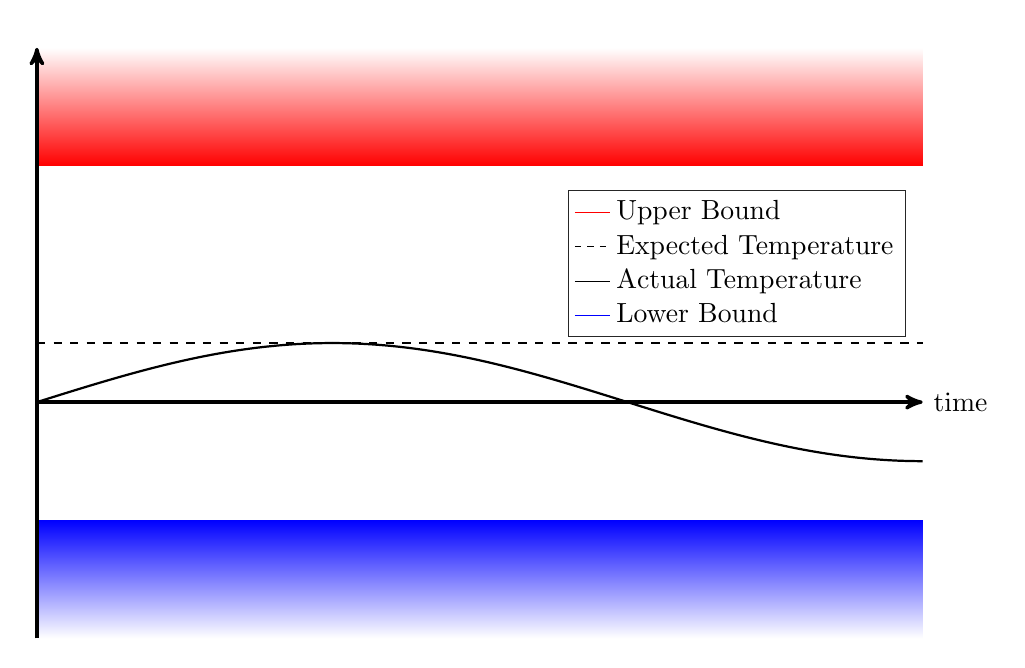
\begin{tikzpicture}[
        %We set the scale and define some styles
        scale=0.75,
        axis/.style={very thick, ->, >=stealth'},
        important line/.style={thick},
        dashed line/.style={dashed, thick},
        every node/.style={color=black,}
     ]

     % Important coordinates are defined
     \coordinate (upper_bound_start) at (0,4);
     \coordinate (upper_bound_stop) at (15,4);
     \coordinate (lower_bound_start) at (0,-2);
     \coordinate (lower_bound_stop) at (15,-2);

     % Everything for x>0
     \begin{scope}
         \shade[bottom color=red, top color=white]
             ($(upper_bound_start)+(0,2)$) rectangle (upper_bound_stop);
     \end{scope}
     %  Everything for x>0
     \begin{scope}
         \shade[bottom color=white, top color=blue]
             ($(lower_bound_start)-(0,2)$) rectangle (lower_bound_stop);
    \end{scope}

     % axis
     \draw[axis] (0,0)  -- (15,0) node(xline)[right] {time};
     \draw[axis] (0,-4) -- (0,6) node(yline)[above] {\SI{}{\celsius}};

	% Sine curve
	\draw[important line] (0,0) sin (5,1);
	\draw[important line] (5,1) cos (10,0);
	\draw[important line] (10,0) sin (15,-1);

	% Expected line
	\draw[dashed line] (0, 1) -- (15, 1);

	% Legend
    \begin{axis}[
    hide axis,
	at={(175, -350)},
    xmin=0,
    xmax=15,
    ymin=-4,
    ymax=6,
    legend style={draw=white!15!black,legend cell align=left}
    ]
     \addlegendimage{red}
     \addlegendentry[scale=1/0.75]{Upper Bound};
     \addlegendimage{black, dash pattern=on 3pt off 3 pt}
     \addlegendentry[scale=1/0.75]{Expected Temperature};
     \addlegendimage{black}
     \addlegendentry[scale=1/0.75]{Actual Temperature};
     \addlegendimage{blue}
     \addlegendentry[scale=1/0.75]{Lower Bound};
    \end{axis}

\end{tikzpicture}

\caption{Theoretical error prone data of a temperature sensor.}
\label{f:simple-boundary}
\end{figure}

The only way to improve error detection would be to not only define multiple sections, like a normal, warning and hazardous limit, but to shape these limits accordingly. Creating shaped limits would have to be specifically set and known beforehand and require the expert knowledge of a human operator. And especially with non-linear values, this might be quite difficult.

\subsection{Out-of-Limit Checks}
The above described boundaries can be narrowed down if the behaviour of the payload as well as the environment of the \ac{spc} and its component arrangement are known. Then one could even shape any arbitrary waveforms to fit the sensor data. But for most cases, the space environment can neither be exactly reproduced nor modelled and simulated on ground with manageable effort. Furthermore, modelling and simulating might be highly expensive and time consuming. And the result in the end would still be a simple boundary not accounting for any possible uncritical - but anomalous - changes.

%\bigbreak

%Therefore we need a technique which is easy and effortless to apply.

\subsection{Human Operators}
Humans can analyse data rather easily and spot outliers as well as larger deviations from repetitive patterns without much knowledge of the particular domain. 

But this bears many problems. First, the data pool is much too large and hence time consuming. Seconding, anomalies might be overlooked in big data pools. The third and sometimes very crucial problem is the delay between acquirement of data and analysis on ground. This also adds to the delay which might be caused by large intervals between ground contact times or just by the sheer distance for deep space missions. %Here a really sophisticated solution for autonomy and automation has to applied to make Mars missions work \cite{mars}. 

%\bigbreak

%As a consequence, the needed technique has to reduce human operator time by precisely distinguishing between normal and anomalous behaviour.

\section{Recent Research}
Most of the recent research and the latest ideas involve machine learning. In the \ac{athmos} research project \cite{athmos} \cite{athmos-sub}, done by DLR at the \ac{gsoc}, a deep neural network combined with an anomaly detection algorithm is developed. \newline
The approach is to have multiple processing, detection and extraction layers which are then combined in the end to get one final result.

An overview of this detection, starting from the raw input and ending in an anomaly detection result is given in figure \ref{f:athmos_anomaly}. The telemetry data is fed into two different modules, a neural network on the left and a \enquote{Feature-Vector Calculator} on the right. The Feature-Vector Calculator features a simple auto-encoder, which de-noises the input and represents a compressed form of the raw data. The neural network is trained to predict future data from the current input data. In other words, the neural network creates a forecast from actual data and compares it with the core features extracted by the Feature-Vector Calculator. From there a deviation score can be calculated.

\begin{figure}[htb]
\centering
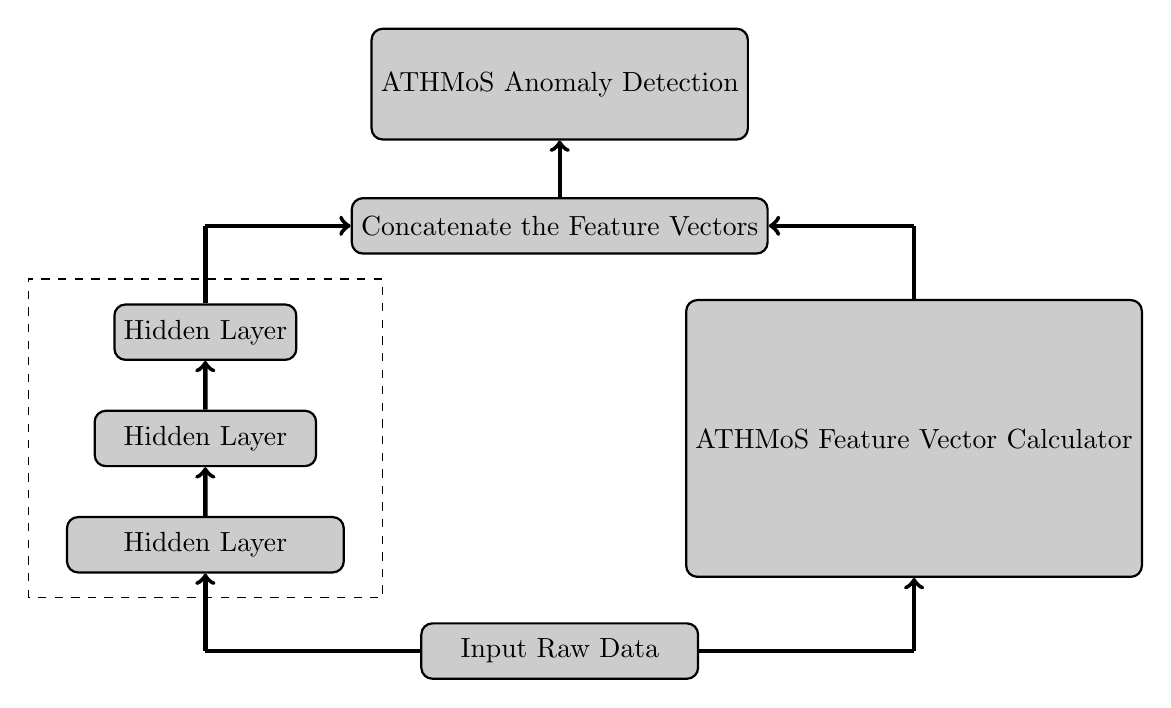
\begin{tikzpicture}[
    block/.style={
      rectangle,
      draw=black,
      thick,
      fill=black!20,
      align=center,
      rounded corners,
      minimum height=2em
    },
    scale=0.9
]

\node[block,minimum height=4em] (aad) at (0,5) {ATHMoS Anomaly Detection};
\node[block] (ctfv) at (0,3) {Concatenate the Feature Vectors};

\draw[->,ultra thick,scale=1.5] (ctfv) -- (aad);

\draw[dashed] (-7.5,-2.25) rectangle (-2.5,2.25);

\node[] (hl) at (-5,3) {};
\node[block, minimum width=6em] (hl3) at (-5,1.5) {Hidden Layer};
\node[block, minimum width=8em] (hl2) at (-5,0) {Hidden Layer};
\node[block, minimum width=10em] (hl1) at (-5,-1.5) {Hidden Layer};

\draw[ultra thick,scale=1.5] (hl3.north) -- (hl.center);
\draw[->,ultra thick,scale=1.5] (hl.center) -- (ctfv.west);
\draw[->,ultra thick,scale=1.5] (hl2) -- (hl3);
\draw[->,ultra thick,scale=1.5] (hl1) -- (hl2);

\node[] (edge) at (5,3) {};
\node[block, minimum height=10em] (afvc) at (5,0) {ATHMoS Feature Vector Calculator};
\draw[ultra thick,scale=1.5] (afvc.north) -- (edge.center);
\draw[->,ultra thick,scale=1.5] (edge.center) -- (ctfv.east);

\node[] (edge1) at (5,-3) {};
\node[] (edge2) at (-5,-3) {};
\node[block, minimum width=10em] (ird) at (0,-3) {Input Raw Data};

\draw[ultra thick,scale=1.5] (ird.east) -- (edge1.center);
\draw[->,ultra thick,scale=1.5] (edge1.center) -- (afvc.south);

\draw[ultra thick,scale=1.5] (ird.west) -- (edge2.center);
\draw[->,ultra thick,scale=1.5] (edge2.center) -- (hl1.south);

\end{tikzpicture}

\caption{\ac{athmos} anomaly detection \cite[p. 8]{athmos}.}
\label{f:athmos_anomaly}
\end{figure}

	\subsection{Automated Telemetry Health Monitoring System (ATHMoS)}
	One example for the anomaly detection technique provided by the authors, was first employed at TET-1 satellite \cite{tet}. Here it was possible to detect an anomaly on a reaction wheel before any boundary detection would have given an alarm \cite[p. 11f]{athmos-sub}.
	
	As this technique is still under development, no hard numbers can be put on the performance. But \ac{athmos} did show that its technique is in general able to work with telemetry in a correct way to predict it in a time frame of 4.5 hours with high accuracy. Along with the distinction between high and low priority anomalies, there is already a benefit regarding satellite health monitoring.

\section{Machine Learning}
\label{c:new_techniques}
New ideas and promising techniques mainly involve \acf{ml}, featuring specifically neural networks. \ac{ml} itself has been in development for many decades. Only in the last decade, computers have become powerful enough to be able to run complex and big neural networks. Hence, using machine learning as a tool for automation and autonomy on \ac{spc} has become an interesting approach for research \cite{ai-dlr-survey}. \newline 
One advantage of \ac{ml} is that it doesn't require as much domain knowledge as statistical methods. Second, statistical methods are not able to process sequential context, which is important when the environment and therefore the data context changes. And third, in general, neural networks can be used to approximate any function, giving them more possible use cases than statistical methods.

As a first step we will here shortly discuss rather simple, but yet powerful, ideas which will later be analysed regarding their performance. These ideas include the \acf{knn}, \acf{aec}, \acf{svm} and \acf{lstm}.

	\subsection{Nearest Neighbour}
	The \ac{knn} algorithm \cite[p. 168ff]{ai-example} is one of the most trivial and simplest ways to divide datasets into groups. It can be used on labelled as well as unlabelled datasets. In the unlabelled case, a margin between groups has to be defined. 
	
\bigbreak

To put the samples into various groups, the distances $\mathbf{D}$ among them has to be calculated:

\begin{equation*}
d_{ij} (P_i, P_j) = \sqrt{(x_i - x_j)^2 + (y_i - y_j)^2}
\end{equation*}	

All points within a certain distance $\left( d_{ij} < \xi \right)$ can form a group and extend this group if they have enough neighbours in their vicinity. If one point has not enough neighbours to form a group of its own, it will be put into a \enquote{noise} group. In figure \ref{f:3_DBSCAN} the execution of a \ac{knn} algorithm is shown. The data has been split into two groups (blue and red) and grey noise points.

\begin{figure}[H]
\centering
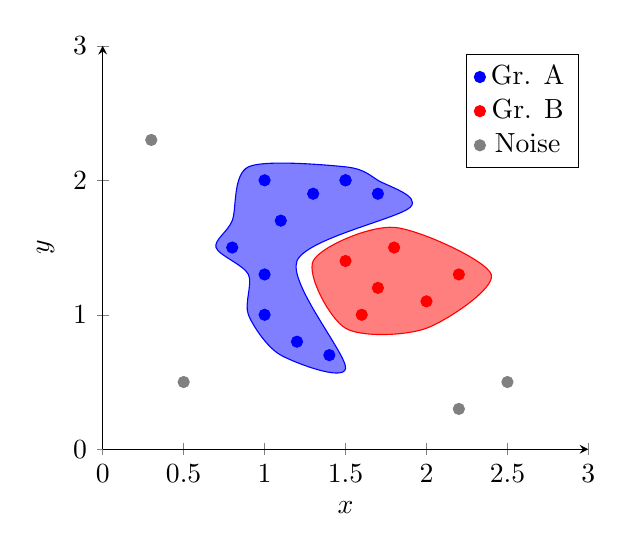
\begin{tikzpicture}
	\begin{axis}[
		xlabel=$x$,
		ylabel=$y$,
		axis x line=bottom,
		axis y line=left,
		ymin=0,
		ymax=3,
		xmin=0,
		xmax=3,
		scale=0.9
]

	\addlegendentry{Gr. A}
	\addplot[only marks, mark=*,color=blue] coordinates {
		(1.4, 0.7) [1]
		(1.2, 0.8) [1]
		(1, 1) [1]
		(1, 1.3) [1]
		(0.8, 1.5) [1]
		(1.1, 1.7) [1]
		(1.3, 1.9)
		(1.5, 2.0)
		(1.5, 2.0)
		(1.0, 2.0)
		(1.7, 1.9)
};

\addlegendentry{Gr. B}
\addplot[only marks, color=red, mark=*] coordinates {
		(1.5, 1.4)
		(1.7, 1.2)
		(1.6, 1.0)
		(2.0, 1.1)
		(2.2, 1.3)
		(1.8, 1.5)
};

\addlegendentry{Noise}
\addplot[only marks, color=gray, mark=*] coordinates {
	(0.5, 0.5)
	(0.3, 2.3)
	(2.5, 0.5)
	(2.2, 0.3)
};

\addplot[smooth cycle, no marks,color=blue,fill=blue, fill opacity=0.5] coordinates {
		(1.5, 0.6)
		(1.1, 0.7)
		(0.9, 1)
		(0.9, 1.3)
		(0.7, 1.5)
		(0.8, 1.7)
		(0.9, 2.1)
		(1.5, 2.1)
		(1.7, 2.0)
		(1.9, 1.8)
		(1.2, 1.4)
};%|- (axis cs:1.2,1.4) -- cycle;

\addplot[smooth cycle, no marks,color=red,fill=red, fill opacity=0.5] coordinates {
		(1.3, 1.4)
		(1.5, 0.9)
		(2.0, 0.9)
		(2.4, 1.3)
		(1.8, 1.65)
};%|- (axis cs:1.8,1.7) -- cycle;

	\end{axis}

\end{tikzpicture}

\caption{k-nearest-neighbour algorithm \enquote{DBSCAN} creates two groups (blue and red) and grey noise points.}
\label{f:3_DBSCAN}
\end{figure}
	
	The computational cost in the standard case is for $N$ samples $\mathcal{O} (N)$. This can be brought down to $\mathcal{O} (\log N)$ with a binary tree and to $\mathcal{O} (1)$ with a hash table \cite[p. 739]{ai-modern}.	

	%TODO Mention that this is not really learning and not supported, therefore we dont use it

	\subsection{Auto-Encoder}
	\acfp{aec} are neural networks for extracting features out of a dataset by the means of encoding the values in a smaller space and decoding it back to the original representation. They have been already used to detect anomalies in various ways \cite{auto-enc-1}\cite{auto-enc-2}\cite{anomaly-basic}. \newline	
	In detail, an \ac{aec} takes the data input vector $\mathbf{x}$, which is then transformed by a trainable weight matrix $\mathbf{W}$ into the hidden layer $\mathbf{h}$. This step is called \enquote{encoding}. The size of $\mathbf{h}$ corresponds to the number of nodes in the layer and is usually smaller than the input in the case of \acp{aec}. The smaller vector $\mathbf{h}$ is then reverse transformed into a vector $\mathbf{y}$ of the same size as the input vector. This step is called \enquote{decoding}. Ideally this should reproduce the previously given input data $\mathbf{x}$. Mathematically written this yields:
	
\begin{align*}
\text{Encoding} & & \mathbf{h} = \mathbf{W}_1\cdot \mathbf{x} \\
\text{Decoding} & & \mathbf{y} = \mathbf{W}_2\cdot \mathbf{h} \\
\end{align*}
	
	This can of course be build with multiple hidden layers. Each layer is then mirrored to give a final output $\mathbf{y}$ equal to the input $\mathbf{x}$. As a general result, the auto-encoder only learns the essential features of the data to recreate the given input. \newline	
	To find anomalies in the end, one has to compare the input vector $\mathbf{x}$ with the output vector $\mathbf{y}$ to calculate any discrepancy.
	
	This basically means, an Auto-Encoder is able to learn a representation of features in a given dataset. Hence it can be used to detect all kinds of features and outliers that were not present before in the particular input from the dataset.
	%Additionally, this method can be used to de-noise the input data.
	The computational cost depends linearly on the number of chosen layers and quadratically on their number of nodes as well as the number of input samples in the given time frame. This totals to a performance of $\mathcal{O} (N^2)$.
	
	\subsection{Support Vector Machines}
	\acfp{svm} \cite[p. 744ff]{ai-modern} are not trivial, but yet quite powerful. They mainly work for separating labelled datasets, but they can also be used in the unsupervised unlabelled case for anomaly detection \cite{one-class-svm}. They work by interpreting every datapoint itself as a vector. Based on that, a boundary line described by a normal vector $\mathbf{w}$ can be drawn to separate these datapoints in a dataset into positive and negative examples:
	
	\begin{equation*}
	y = \mathbf{x}\cdot\mathbf{w} + b = \begin{cases}
	-1 & \text{negative} \\
	\pm 0 & \text{boundary} \\
	+1 & \text{positive} 
	\end{cases}
	\end{equation*}
	
	For datasets that cannot be linearly separated, the dimensionality of the evaluation can be increased with a kernel function. This again can be reduced back with a principal-component-analysis to save computation time. The overall computational cost for finding the boundary line (in training) highly depends on the used optimization algorithm as this is a non-linear optimization problem. For later queries in an already trained network, the cost is linear to the input vector length.
	
	\subsection{Long Short-Term Memory}
	\acfp{lstm} were introduced by Sepp Hochreiter \cite{lstm} out of the need to create a recurrent neural network, that works with learned long-term input as well as recent short-term input. Especially taking into account the chronological order of the various inputs. \newline
	Conventional recurrent networks do suffer from error back propagation with large time delays, where the error gradient would either completely vanish, explode or in some cases even oscillate. This was solved by \enquote{enforcing constant (thus neither exploding nor vanishing) error flow through internal states of special units} \cite[p. 1f]{lstm}. \newline
	In figure \ref{f:lstm} a \ac{lstm} module with its special internal units is shown. Each gate in the module can be thought of as a single neuron. There are the output gate $o_t$, forget gate $f_t$ and input gate $i_t$. In the very middle is the cell $c_t$ memorizing the state. The big S-circles represent the activation functions, like the sigmoid function. The small X-circles are for point-wise multiplication operations.
		
	\acp{lstm} have become interesting only in the recent years with increasing computational power and memory, and the possibility of using huge datasets.
	
	One very important area for \ac{lstm} networks is text and speech recognition. Here the context of a sentence depends on all the sentences said or written before as well as the actual sentence presented. Thus their popularity and use has vastly increased over the recent years.
	
	They have also been proven to be useful in space mission as Kyle Hundman et al. at NASA JPL have shown on two Mars missions \cite{sc-lstm-detection}. With an anomaly detection system built on the basis of an \ac{lstm} they were able to label anomalies in telemetry data in the Mars Science Laboratory (MSL)\footnote{Also known as \enquote{Curiosity}} and the Soil Moisture Active Passive (SMAP) satellite.	
	
	\begin{figure}[htb]
	\centering
	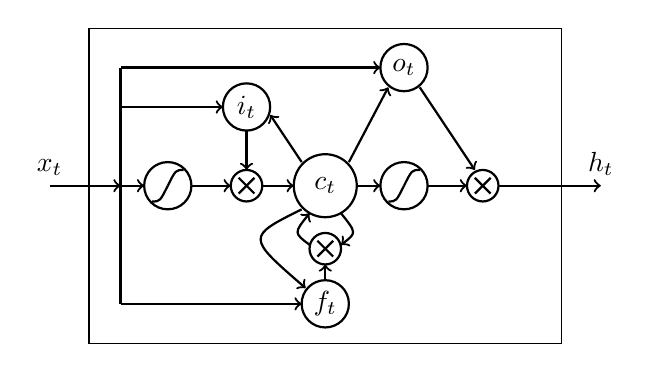
\begin{tikzpicture}

%% Outer box %%
\draw (0,0) rectangle (6,4);

%% Connection arrows %%
% left to right %
\draw[->, thick] (-0.5, 2) -- (0.4, 2) node[pos=0, above] {$x_t$};
\draw[->, thick] (0.4, 2) -- (0.7, 2);

\draw[->, thick] (1.3, 2) -- (1.8, 2);
\draw[->, thick] (2.2, 2) -- (2.6, 2);

\draw[->, thick] (3.4, 2) -- (3.7, 2);
\draw[->, thick] (4.3, 2) -- (4.8, 2);

\draw[->, thick] (5.2, 2) -- (6.5, 2) node[pos=1, above] {$h_t$};

% interconnection %
\draw[thick] (0.4, 3.5) -- (0.4, 0.5);
\draw[thick,->] (0.4, 3.5) -- (3.7, 3.5);
\draw[thick,->] (0.4, 0.5) -- (2.7, 0.5);
\draw[thick,->] (0.4, 3) -- (1.7, 3);

\draw[thick,->] (2, 2.7) -- (2, 2.2);
\draw[thick,->] (2.7, 2.3) -- (2.3, 2.9);
\draw[thick,->] (3.3, 2.3) -- (3.8, 3.25);

\draw[thick,->] (4.2, 3.25) -- (4.9, 2.2);

\draw[thick,->] (3, 0.8) -- (3, 1);

\draw[thick,->] (2.7, 1.7) .. controls (2, 1.35) .. (2.75, 0.7);

\draw[thick,->] (2.8, 1.25) .. controls (2.6, 1.4) .. (2.8, 1.65);
\draw[thick,->] (3.2, 1.65) .. controls (3.4, 1.4) .. (3.2, 1.25);

%% Nodes %%
% Sigmoid left %
\draw[thick] (1, 2) circle (0.3);
\draw[thick] (0.8, 1.8) .. controls (0.9, 1.8) .. (1, 2);
\draw[thick] (1, 2) .. controls (1.1, 2.2) .. (1.2, 2.2);

% Multiplication left %
\draw[thick] (2, 2) circle (0.2);
\draw[thick] (1.9, 1.9) -- (2.1, 2.1);
\draw[thick] (2.1, 1.9) -- (1.9, 2.1);

\draw[thick] (3,2) circle(0.4) node {$c_t$};

% Sigmoid right %
\draw[thick] (4, 2) circle (0.3);
\draw[thick] (3.8, 1.8) .. controls (3.9, 1.8) .. (4, 2);
\draw[thick] (4, 2) .. controls (4.1, 2.2) .. (4.2, 2.2);

% Multiplication right %
\draw[thick] (5, 2) circle (0.2);
\draw[thick] (4.9, 1.9) -- (5.1, 2.1);
\draw[thick] (5.1, 1.9) -- (4.9, 2.1);

% input gate %
\draw[thick] (2, 3) circle (0.3) node {$i_t$};

% output gate %
\draw[thick] (4, 3.5) circle (0.3) node {$o_t$};

% forget gate %
\draw[thick] (3, 0.5) circle (0.3) node {$f_t$};
\draw[thick] (3, 1.2) circle (0.2);
\draw[thick] (2.9, 1.1) -- (3.1, 1.3);
\draw[thick] (3.1, 1.1) -- (2.9, 1.3);

\end{tikzpicture}

	\caption{Structure of an \ac{lstm} module. The data $\mathbf{x}_t$ propagates through activation functions (S-circle), is convoluted (X-circle) and gets offset against the internal gates ($i_t$, $o_t$ and $f_t$) to the output $\mathbf{h}_t$.}
	\label{f:lstm}
	\end{figure}

	In contrast to \acp{svm} as well as basic neural networks, \acp{lstm} can be used to either categorize or predict future output, depending on the last layer. Hence it can be used to input telemetry data and make future predictions including past and recent changes. As a result, these predictions can be tested against simple boundaries to check if a value is about to cross the limit in the near future.